\documentclass[11pt]{report}
\usepackage[french]{babel}
\usepackage[utf8]{inputenc}
\usepackage[T1]{fontenc}
\usepackage[top = 2cm, bottom = 2cm, left = 1cm, right = 1cm]{geometry}
\usepackage{fancyvrb}
\usepackage{mathalfa}
\usepackage{amsfonts}
\usepackage[table]{xcolor}
\usepackage{amsmath}
\usepackage{graphicx}
\usepackage{listings}
\usepackage{color}
\usepackage{comment}

\fontfamily{ptm}

\begin{document}

\selectfont

\noindent
\textbf{Hachem BENYAHIA}
~\\
\textbf{Cristian GHITU}

~\\
\begin{center}
\section*{Compte-rendu IA04 - TD4 ~\\ Simulation et Environnement ~\\ Le Sudoku}

~\\
\rule{\textwidth}{1pt}
\end{center}

~\\\\
\textbf{1. Quels sont les rôles de chaque type d'agent ?}

~\\
Il y a trois types d'agents au total : 

~\
\begin{enumerate}
\item Le type \textbf{Agent d'environnement} (\verb|EnvironmentAgent| dans le code) : stocke la matrice qui représente la grille de Sudoku chargée initialement. Il conserve également une version qui correspond à l'état actuel de la matrice en cours de résolution. C'est cet agent qui se charge de recevoir les messages en provenance de la console JADE.

~\
\item Le type \textbf{Agent de simulation} (\verb|SimulationAgent| dans le code) : fais la jonction entre chaque agent d'analyse et l'agent d'environnement. Il se charge de mettre à jour la grille partiellement résolue en fonction des données envoyées par les agents d'analyse. Il envoie périodiquement à une salve de messages aux agents d'analyses contenant la portion à analyser. Il envoie également de temps en temps un message de mise à jour à l'agent d'environnement pour qu'il \textit{update} sa version actuelle de la grille (partiellement résolue).

~\
\item Le type \textbf{Agent d'analyse} (\verb|AnalysisAgent| dans le code) : 27 instances traitent chacune leur partie de ligne et déduisent les possibilités pour chaque case traitée.
\end{enumerate}

~\\
\textbf{2. Quelles sont les tâches de chaque type d'agents (en termes de behaviours simples et
composites) ?}

~\\
\verb|EnvironmentAgent| possède 2 behaviours : 

~\
\begin{enumerate}
\item \verb|ReceiveFromConsoleEnvironmentBehaviour| : comme son nom l'indique, ce behaviour gère les messages en provenance de la console JADE. Principalement, il peut afficher la grille partiellement résolue actuelle et lire une nouvelle grille (ce qui redémarrera totalement le programme et enchainera une nouvelle série de résolutions). Ce behaviour hérite de \verb|CyclicBehaviour|.

~\
\item \verb|ReceiveFromSimulationEnvironmentBehaviour| : là encore, le nom induit que ce behaviour traite les messages reçus de l'agent de simulation. En effet, ce dernier envoie périodiquement la version la plus à jour de la grille partiellement résolue à l'agent d'environnement.Ce behaviour hérite de \verb|CyclicBehaviour|.
\end{enumerate}

\newpage
\noindent
Étant à la jonction des deux autres types d'agents, \verb|SimulationAgent| est très sollicité et possède   4 behaviours : 

~\
\begin{enumerate}
\item \verb|ReceiveFromAnalysisSimulationBehaviour| : ce behaviour traite les message reçus des agents d'analyse. Quand un agent a terminé son analyse, il renvoie un message à l'agent de simulation. Quand ce dernier reçoit cette réponse, il décrémente le nombre de messages qu'il attends (sur les 27 messages initiaux envoyés). Ce behaviour hérite de \verb|CyclicBehaviour|.

~\
\item \verb|SimulationToEnvironmentBehaviour| : ce behaviour envoie périodiquement à l'agent d'environnement la version actuelle de la grille partiellement résolue. Ce behaviour hérite de \verb|TickerBehaviour|.

~\
\item \verb|SimulationToAnalysisBehaviour| : l'agent de simulation utilise ce behaviour pour envoyer périodiquement une salve de messages aux 27 agents d'analyses pour qu'ils traitent la portion de grille qui les concerne. Ce behaviour hérite de \verb|TickerBehaviour|.

~\
\item \verb|ReceiveFromEnvironmentSimulationBehaviour| : comme son nom l'indique, ce behaviour traite les messages reçus de l'agent d'environnement. En fait, on pourrait penser qu'il ne s'active qu'une seule fois, mais il est possible en fait de modifier la grille originale bien que le programme soit déjà en cours d'une résolution d'une grille, donc ce behaviour n'est pas un \verb|OneShotBehaviour| mais bien un \verb|CyclicBehaviour|. Son rôle est de mettre à jour la grille à résoudre dans l'agent de simulation.
\end{enumerate}

~\\
\verb|AnalysisAgent| possède quant à lui 1 behaviour : 

~\
\begin{enumerate}
\item \verb|ReceiveFromSimulationAnalysisBehaviour| : ce behaviour traite les messages reçus de la part de l'agent de simulation. Les messages en question sont les parties de la grille à analyser (une partie par agent d'analyse). Ce behaviour hérite de \verb|CyclicBehaviour|.
\end{enumerate}

~\\
\textbf{3. Quel sont les types des messages échangés (request, inform, subscribe, etc.), leur
utilité et leur contenu ?}

~\\
La console JADE communique avec l'agent d'environnement via des messages de type \verb|ACLMessage.REQUEST|. La communication est unidirectionnelle, l'agent d'environnement n'envoie jamais de messages à la console JADE. Ces messages ont pour but soit de demander un affichage de la grille partiellement résolue actuelle, soit de charger une nouvelle grille à résoudre.

~\\
L'agent d'environnement et l'agent de simulation communiquent entre eux par des messages de type \verb|ACLMessage.INFORM|. Ce type est réservé à leur communication. Ainsi, si l'agent de simulation reçoit un \verb|ACLMessage.INFORM|, il sait automatiquement que le message provient de l'agent d'environnement. Les messages de l'agent d'environnement à l'agent de simulation sont en réponse à la requête de chargement d'une nouvelle grille en provenance de la console. Les messages de l'agent de simulation à l'agent d'environnement sont des mises à jour de la grille partiellement résolue actuelle (mettre à jour la version de l'agent d'environnement).

~\\
L'agent de simulation et les agents d'analyses communiquent entre eux par des messages de type \verb|ACLMessage.AGREE|. Ce type est réservé à leur communication. Ainsi, si l'agent de simulation reçoit un \verb|ACLMessage.AGREE|, il sait automatiquement que le message provient d'un agent d'analyse. Les messages de l'agent de simulation vers les agents d'analyses sont les envois périodiques de parties de la grille à être analysés. Les messages dans l'autre sens sont des réponses des agents d'analyses quand ils ont terminé d'analyser leur partie de grille.

\newpage
Voici un schéma qui complète la réponse :

~\\
\begin{figure}[h]
\begin{center}
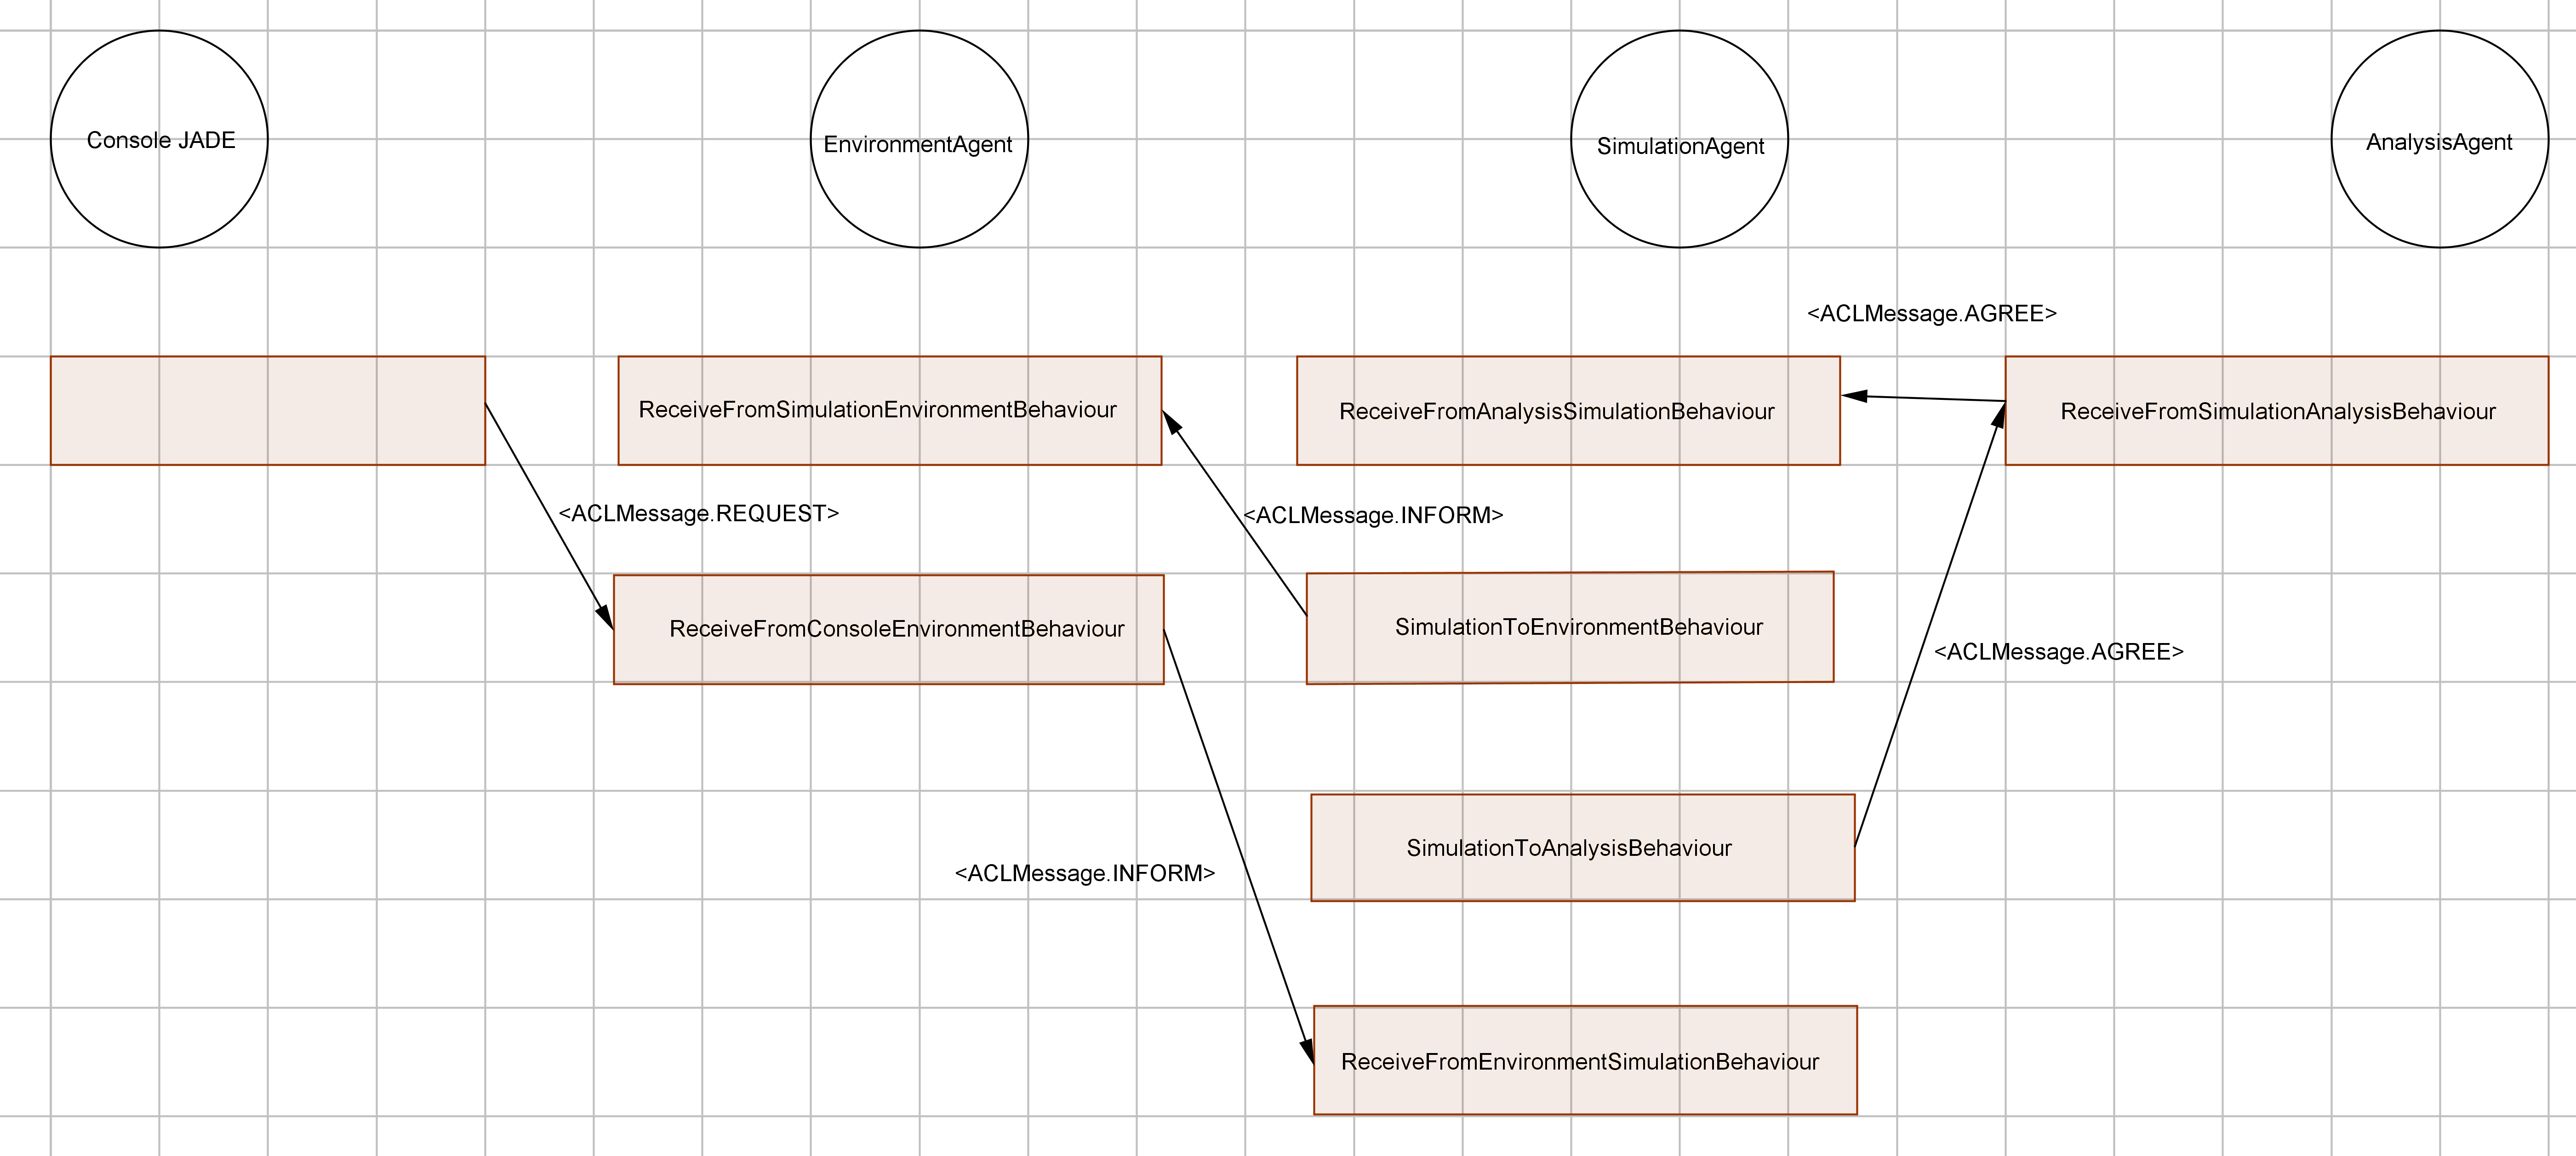
\includegraphics[width=\textwidth]{schema.png}
\end{center}
\end{figure}

~\\
\textbf{4. En supposant que les agents d'analyse sont situés sur différentes stations, la résolution
est-elle encore possible ?}

~\\
Dans JADE, une connexion à une plate-forme est en fait une connexion à un conteneur qui se trouve sur une plate-forme différente via le fichier de configuration \textbf{properties}. Si on crée un conteneur secondaire par station et que dans un conteneur primaire on instancie ces conteneurs étrangers (en leur associant donc à chaque fois le bon fichier \textbf{properties}), on peut a priori rapatrier les données localement.
\end{document}